% Mini Research Problem -- Artificial Intelligence (Advanced Topics in AI & ML)
% Explainable AI for Network Intrusion Detection
% Compile: pdflatex mrp_xai_nids.tex  (twice)
\documentclass[10pt,aspectratio=169]{beamer}

\usepackage[T1]{fontenc}
\usepackage[utf8]{inputenc}
\usepackage{lmodern}
\usepackage{booktabs}
\usepackage{graphicx}
\usepackage{tikz}
\usetikzlibrary{arrows.meta, positioning}
\usepackage{hyperref}
\hypersetup{hidelinks}

% auto-generated by src/report.py - do not edit
\newcommand{\nTrain}{125\,973}
\newcommand{\nTest}{22\,544}
\newcommand{\nCols}{122}
\newcommand{\nFields}{41}
\newcommand{\rfVal}{99.9}
\newcommand{\rfTest}{74.8}
\newcommand{\mlpVal}{99.6}
\newcommand{\mlpTest}{79.4}
\newcommand{\recDoS}{77}
\newcommand{\recProbe}{60}
\newcommand{\recRTL}{7}
\newcommand{\recUTR}{7}
\newcommand{\nExplained}{2467}
\newcommand{\aopcShap}{0.69}
\newcommand{\aopcLime}{0.44}
\newcommand{\aopcRand}{0.22}
\newcommand{\dropTopThree}{0.61}
\newcommand{\nFaith}{120}
\newcommand{\stabLime}{0.66}
\newcommand{\stabShap}{1.00}
\newcommand{\msTree}{47}
\newcommand{\msLime}{74}
\newcommand{\msKernel}{31}
\newcommand{\jacSL}{0.41}
\newcommand{\rhoSL}{-0.12}
\newcommand{\corrAlign}{0.90}
\newcommand{\liftDoS}{1.45}
\newcommand{\shareDoS}{64}
\newcommand{\baseDoS}{44}
\newcommand{\liftProbe}{1.25}
\newcommand{\shareProbe}{58}
\newcommand{\baseProbe}{46}
\newcommand{\liftRTL}{1.09}
\newcommand{\shareRTL}{58}
\newcommand{\baseRTL}{54}
\newcommand{\liftUTR}{0.83}
\newcommand{\shareUTR}{26}
\newcommand{\baseUTR}{32}


% ---------------------------------------------------------------- plain style
\usetheme{default}
\usecolortheme{dove}
\setbeamertemplate{navigation symbols}{}
\setbeamertemplate{itemize items}[circle]
\setbeamertemplate{itemize subitem}{--}
\definecolor{accent}{HTML}{1B4F72}
\setbeamercolor{frametitle}{fg=accent}
\setbeamercolor{structure}{fg=accent}
\setbeamerfont{frametitle}{series=\bfseries,size=\large}
\setbeamerfont{footline}{size=\tiny}
\setbeamertemplate{footline}{%
  \hfill\usebeamerfont{footline}\color{gray}%
  XAI for Network Intrusion Detection \quad
  \insertframenumber/\inserttotalframenumber\hspace{2ex}\vspace{1ex}}
\setlength{\parskip}{2pt}

\newcommand{\f}[1]{{\small\texttt{#1}}}
\newcommand{\link}[2]{\href{#1}{\color{accent}\underline{#2}}}

\title{\bfseries Explainable AI for Network Intrusion Detection}
\subtitle{Are SHAP explanations of an IDS faithful, stable, and consistent with
network protocol semantics?}
\author{Mini Research Problem -- Advanced Topics in AI \& ML}
\date{}

\begin{document}

{\setbeamertemplate{footline}{}
\begin{frame}[plain]
  \titlepage
  \vspace{-1.2em}
  \centering\small
  Code and reproduction scripts:\\
  \link{https://github.com/Wangzx9908/ai-hw-SUMMER-2026-MRP}{github.com/Wangzx9908/ai-hw-SUMMER-2026-MRP}
\end{frame}}

% ============================================================== 1. tl;dr
\begin{frame}{tl;dr}
\small
\begin{block}{Motivation}
An ML-based IDS outputs \emph{block} or \emph{allow}. A network engineer cannot
act on that: was the flow dropped because of a half-open TCP state, a zero-byte
payload, or service fan-out? Without a reason there is no way to tell a true
detection from a false positive that just killed a production service.
\end{block}
\vspace{-0.3em}
\begin{block}{Main idea}
Train flow classifiers on NSL-KDD (\nTrain{} train / \nTest{} unseen test
flows), attribute every decision with SHAP, sum attributions over one-hot
groups back to the \nFields{} protocol fields, and then \emph{test the
explanations themselves}: domain consistency, faithfulness, stability, cost.
\end{block}
\vspace{-0.3em}
\begin{block}{Results}
\begin{itemize}\itemsep1pt
  \item Learned logic matches textbook signatures: DoS $\to$ \f{count}, \f{flag=REJ};
        Probe $\to$ \f{src\_bytes}=0, \f{diff\_srv\_rate}; R2L $\to$ \f{hot}, \f{logged\_in}.
  \item Domain alignment predicts generalisation: lift \liftDoS{} (DoS) $\to$ \liftUTR{} (U2R),
        correlation \corrAlign{} with per-family recall on unseen attacks.
  \item SHAP is markedly more faithful than LIME (AOPC \aopcShap{} vs \aopcLime{}, random \aopcRand{})
        and perfectly reproducible (\stabShap{} vs \stabLime{} top-5 Jaccard).
  \item \msTree{}\,ms per explained flow $\Rightarrow$ viable in a SOC console, not inline at line rate.
\end{itemize}
\end{block}
\end{frame}

% ============================================================== 2. problem
\begin{frame}{The problem: accuracy hides the failure mode}
\small
\begin{columns}[T]
\begin{column}{0.53\textwidth}
\begin{tabular}{lcc}
\toprule
 & \textbf{same-distribution} & \textbf{official KDDTest+} \\
 & held-out split & (17 novel attacks) \\
\midrule
Random Forest & \rfVal\,\% & \rfTest\,\% \\
MLP (64--32)  & \mlpVal\,\% & \mlpTest\,\% \\
\bottomrule
\end{tabular}

\vspace{0.7em}
Random Forest recall per family on unseen traffic:

\vspace{0.3em}
\begin{tabular}{cccc}
\toprule
DoS & Probe & R2L & U2R \\
\midrule
\recDoS\,\% & \recProbe\,\% & \recRTL\,\% & \recUTR\,\% \\
\bottomrule
\end{tabular}
\end{column}
\begin{column}{0.45\textwidth}
\begin{itemize}\itemsep3pt
  \item A published \rfVal\,\% collapses to \rfTest\,\% once the attack mix
        changes -- the number alone gives no clue where the model went wrong.
  \item R2L / U2R are essentially undetected, yet the aggregate accuracy still
        looks acceptable.
  \item Lecture 09: \emph{interpretability as an ML debugging tool}. We use
        attributions to ask \textbf{which fields the model actually relies on},
        and whether those are the ones a protocol analyst would use.
\end{itemize}
\end{column}
\end{columns}
\end{frame}

% ============================================================== 3. lit review I
\begin{frame}{Literature review (1/2): black-box detectors in security}
\small
\begin{itemize}\itemsep4pt
  \item \textbf{Sommer \& Paxson, IEEE S\&P 2010} -- \emph{Outside the Closed
        World}. ML-based NIDS suffer from a \emph{semantic gap}: an anomaly
        score is not an actionable finding; operators need the reason to
        respond. Still the reference framing for this problem.
  \item \textbf{Arp et al., USENIX Security 2022} -- \emph{Dos and Don'ts of ML
        in Computer Security}. Documents spurious correlations and sampling
        artefacts in security datasets; recommends inspecting learned features
        rather than trusting held-out scores.
  \item \textbf{Tavallaee et al., CISDA 2009} -- NSL-KDD. Removes KDD'99
        duplicates and keeps a test split with attack types absent from
        training, which is exactly the generalisation gap on the previous slide.
  \item \textbf{Rudin, Nature Mach.\ Intell.\ 2019} -- argues for inherently
        interpretable models in high-stakes settings instead of post-hoc
        explanation. Our counter-position: production IDS stacks are already
        ensembles/DL, so post-hoc attribution must at least be \emph{validated}.
  \item \textbf{Doshi-Velez \& Kim, 2017} -- taxonomy of interpretability
        evaluation (functionally / human / application grounded); we stay at the
        functionally-grounded level (proxy metrics, no user study).
\end{itemize}
\end{frame}

% ============================================================== 4. lit review II
\begin{frame}{Literature review (2/2): attribution methods and the gap}
\scriptsize
\begin{tabular}{lccccl}
\toprule
\textbf{Method} & \textbf{Access} & \textbf{Cost/flow} & \textbf{Determ.} & \textbf{Axioms} & \textbf{Source} \\
\midrule
LIME              & black box & $\sim$1k queries & no  & none        & Ribeiro et al., KDD 2016 \\
KernelSHAP        & black box & $10^2$--$10^3$   & no  & Shapley (approx.) & Lundberg \& Lee, NeurIPS 2017 \\
TreeSHAP          & trees     & polynomial, exact & yes & Shapley     & Lundberg et al., Nat.\ MI 2020 \\
Integrated Grad.  & gradients & $\sim$50 passes  & yes & completeness & Sundararajan et al., ICML 2017 \\
LEMNA             & black box & high             & no  & none        & Guo et al., CCS 2018 (security-specific) \\
\bottomrule
\end{tabular}

\vspace{0.9em}
\normalsize\textbf{Applied to intrusion detection}
\vspace{0.2em}
\scriptsize
\begin{itemize}\itemsep2pt
  \item \textbf{Wang et al., IEEE Access 2020} -- SHAP-based framework for IDS on NSL-KDD /
        UNSW-NB15: local and global feature importance per attack class.
  \item \textbf{Mane \& Rao, 2021} -- SHAP + LIME + contrastive explanations on NSL-KDD deep models.
  \item \textbf{Warnecke et al., IEEE EuroS\&P 2020} -- compares LIME/SHAP/LRP/IG on
        security tasks using descriptive accuracy, sparsity, stability, efficiency.
  \item \textbf{Han et al., CCS 2021 (DeepAID)} -- interprets unsupervised deep anomaly
        detectors and feeds the explanation back into the detector.
  \item \textbf{Nadeem et al., IEEE EuroS\&P 2023} -- SoK on XAI for security; notes that most
        papers \emph{display} explanations without validating them.
\end{itemize}
\vspace{0.4em}
\normalsize\textbf{Gap addressed here:} prior IDS work mostly \emph{shows} SHAP plots. We ask
whether the attributions are faithful, reproducible, cheap enough, and aligned
with protocol semantics -- and whether that alignment says anything about
generalisation.
\end{frame}

% ============================================================== 5. approach
\begin{frame}{Approach}
\centering
\resizebox{\textwidth}{!}{%
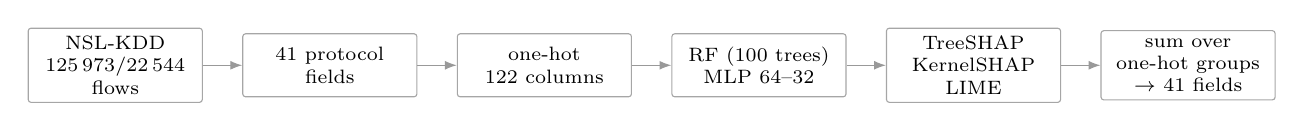
\begin{tikzpicture}[
  node distance=4.2mm and 5mm,
  box/.style={draw=gray!70, rounded corners=1pt, align=center,
              font=\scriptsize, inner sep=3pt, minimum height=8mm,
              text width=20mm},
  ar/.style={-{Latex[length=1.5mm]}, gray!80}]
\node[box] (a) {NSL-KDD\\ \nTrain{}/\nTest{} flows};
\node[box, right=of a] (b) {\nFields{} protocol\\ fields};
\node[box, right=of b] (c) {one-hot\\ \nCols{} columns};
\node[box, right=of c] (d) {RF (100 trees)\\ MLP 64--32};
\node[box, right=of d] (e) {TreeSHAP\\ KernelSHAP\\ LIME};
\node[box, right=of e] (f) {sum over\\ one-hot groups\\ $\to$ \nFields{} fields};
\foreach \x/\y in {a/b, b/c, c/d, d/e, e/f} \draw[ar] (\x) -- (\y);
\end{tikzpicture}}

\vspace{0.6em}
\raggedright\scriptsize
\textbf{Key design decision.} One-hot encoding turns \f{service}, \f{flag},
\f{protocol\_type} into \nCols{} columns, and per-column attributions
(\f{service=ecr\_i}: 0.004) are unusable in an incident report. Shapley values
are additive, so summing over a disjoint group of columns is exactly the
attribution of the original field. All results are reported on the
\nFields{} semantic fields.

\vspace{0.5em}
\textbf{Four experiments on the \nExplained{} explained unseen flows.}
\begin{itemize}\itemsep1pt
  \item \textbf{E1 domain consistency} -- share of attributed mass falling in the
        feature groups (basic / content / time-traffic / host-traffic) that IDS
        literature associates with each family, \emph{fixed before} looking at any output;
        reported as lift over a mass-proportional-to-count baseline.
  \item \textbf{E2 faithfulness} -- deletion test: move the top-$k$ ranked fields to a
        benign reference profile, measure the drop in attack probability (\nFaith{} flows).
  \item \textbf{E3 stability} -- re-explain the same flow 5 times, top-5 Jaccard between runs.
  \item \textbf{E4 cost} -- wall-clock ms per explained flow.
\end{itemize}
\vspace{0.3em}
\textbf{Tools:} \link{https://scikit-learn.org/}{scikit-learn} $\cdot$
\link{https://github.com/shap/shap}{shap 0.52} $\cdot$
\link{https://github.com/marcotcr/lime}{lime 0.2} $\cdot$
data: \link{https://www.unb.ca/cic/datasets/nsl.html}{NSL-KDD (UNB CIC)}
\end{frame}

% ============================================================== 6. global
\begin{frame}{Result 1: global attribution matches protocol intuition}
\centering
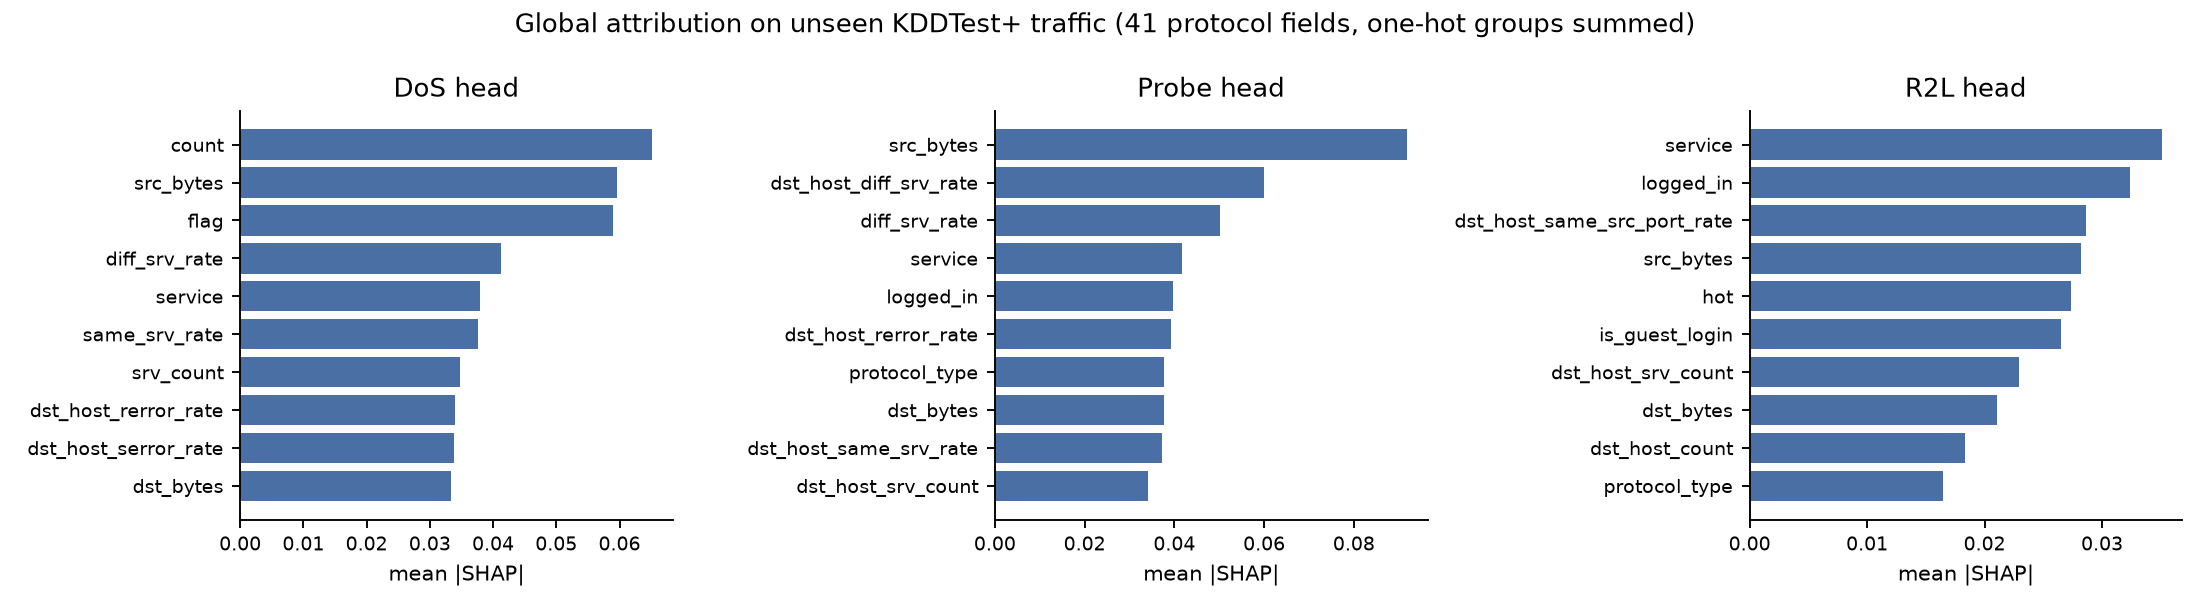
\includegraphics[width=\textwidth]{../figures/global_per_class.png}

\vspace{0.4em}
\raggedright\scriptsize
\begin{itemize}\itemsep1pt
  \item \textbf{DoS}: \f{count}, \f{flag}, \f{srv\_count}, \f{dst\_host\_serror\_rate}
        -- connection volume plus half-open / rejected TCP states, i.e.\ the SYN-flood signature.
  \item \textbf{Probe}: \f{src\_bytes}$\approx$0 with high \f{diff\_srv\_rate} and
        \f{dst\_host\_diff\_srv\_rate} -- empty connections fanned out over many
        services, i.e.\ a port sweep.
  \item \textbf{R2L}: content/authentication fields \f{logged\_in}, \f{hot},
        \f{is\_guest\_login}, \f{service} -- no volumetric signal at all, consistent
        with credential attacks hiding inside single well-formed sessions.
\end{itemize}
\end{frame}

% ============================================================== 7. E1
\begin{frame}{Result 2: alignment with domain knowledge predicts generalisation}
\small
\begin{columns}[T]
\begin{column}{0.46\textwidth}
\centering
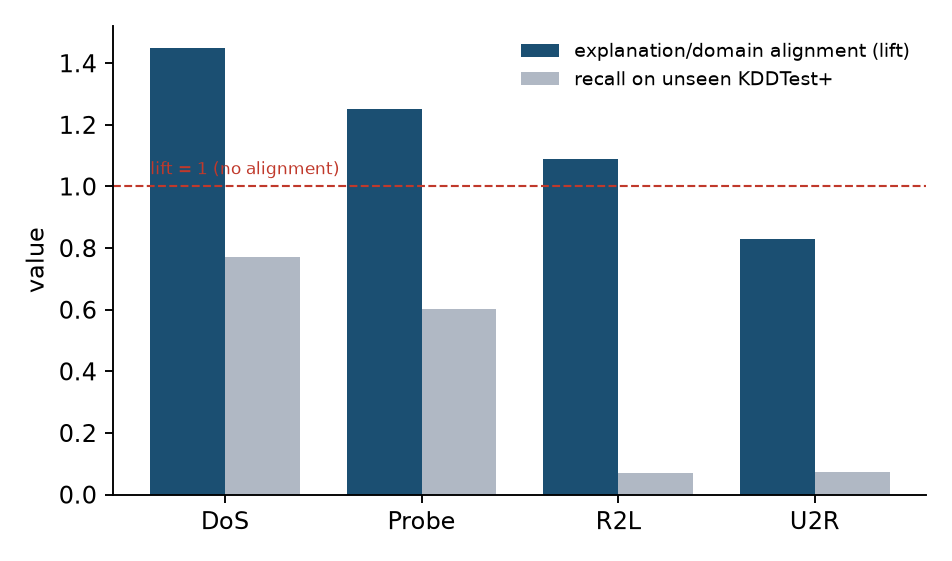
\includegraphics[width=\textwidth]{../figures/alignment_vs_recall.png}
\end{column}
\begin{column}{0.53\textwidth}
\scriptsize
\begin{tabular}{lccc}
\toprule
Family & expected & attributed & lift \\
       & groups   & share      &      \\
\midrule
DoS   & time+basic     & \shareDoS\,\% (base \baseDoS\,\%)   & \liftDoS \\
Probe & time+host      & \shareProbe\,\% (base \baseProbe\,\%) & \liftProbe \\
R2L   & content+basic  & \shareRTL\,\% (base \baseRTL\,\%)   & \liftRTL \\
U2R   & content        & \shareUTR\,\% (base \baseUTR\,\%)   & \liftUTR \\
\bottomrule
\end{tabular}
\vspace{0.8em}
\begin{itemize}\itemsep3pt
  \item For DoS and Probe the model puts \shareDoS\,\% / \shareProbe\,\% of its
        attribution mass on the field groups an analyst would use -- clear lift
        over chance.
  \item For U2R the lift drops \emph{below 1}: the model ignores \f{root\_shell},
        \f{num\_file\_creations} and leans on host-traffic counters instead --
        a shortcut, not a signature.
  \item Alignment lift correlates \corrAlign{} with per-family recall on unseen
        attacks. The explanation exposed \emph{why} R2L/U2R fail before any new
        labelled data was collected.
\end{itemize}
\end{column}
\end{columns}
\end{frame}

% ============================================================== 8. local TP
\begin{frame}{Result 3: a local explanation an engineer can act on}
\small
\begin{columns}[T]
\begin{column}{0.5\textwidth}
\centering
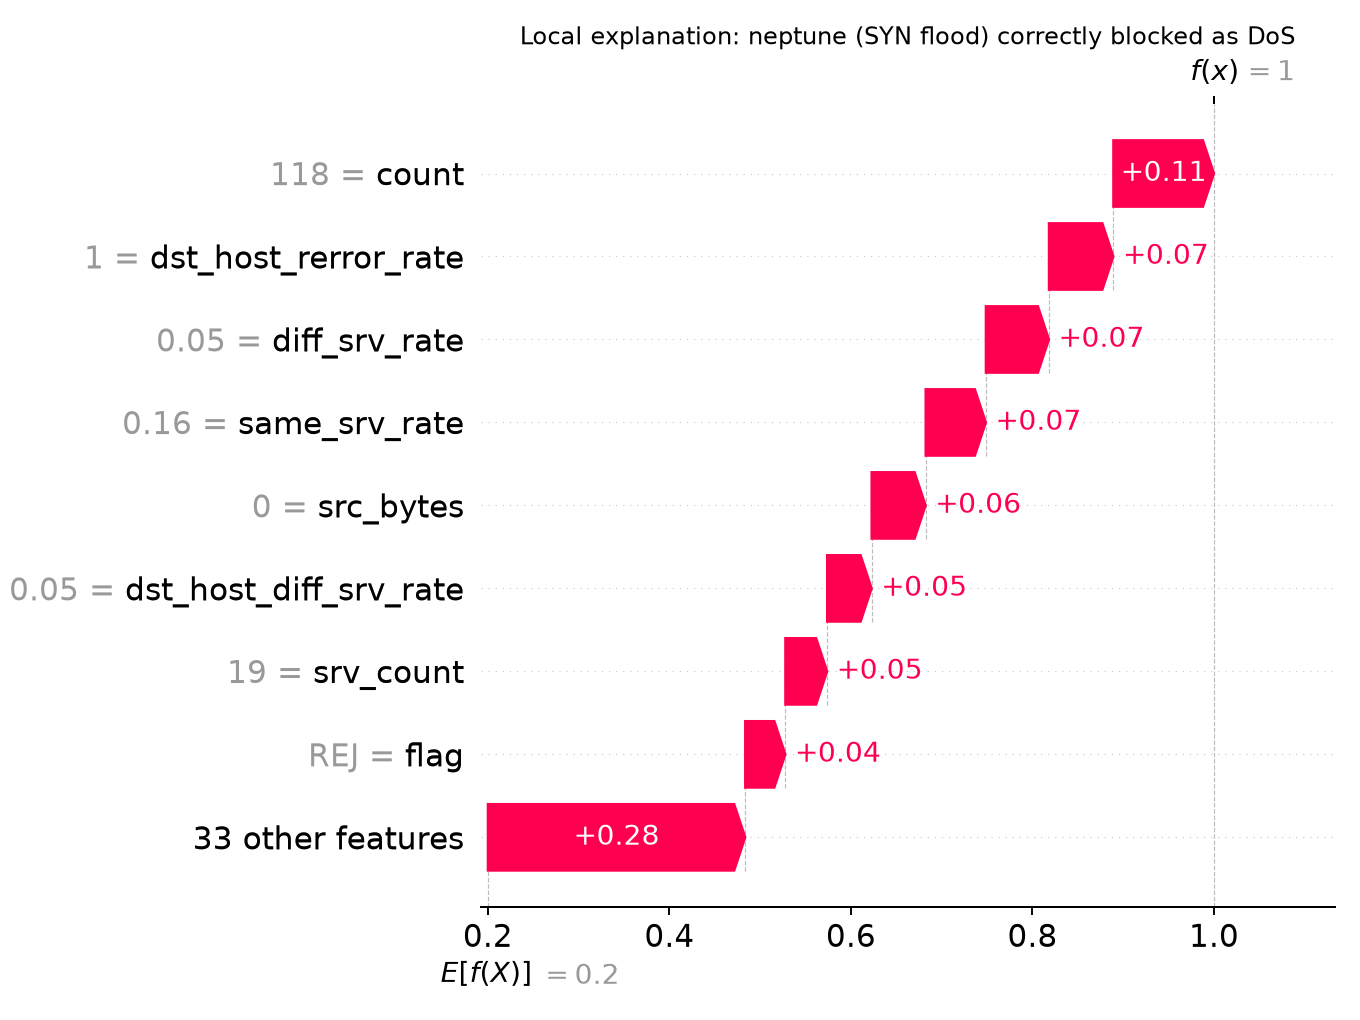
\includegraphics[width=0.98\textwidth]{../figures/local_neptune.png}
\end{column}
\begin{column}{0.48\textwidth}
\scriptsize
One \f{neptune} flow, blocked as DoS with $p=1.00$. Base rate $E[f(x)]=0.20$.

\vspace{0.6em}
Rendered straight from the SHAP vector as a log line:
\vspace{0.3em}

\fbox{\parbox{0.95\linewidth}{\ttfamily\tiny
verdict=DoS p=1.00 because\\
count=118 (+0.111),\\
dst\_host\_rerror\_rate=1.00 (+0.071),\\
diff\_srv\_rate=0.05 (+0.070),\\
same\_srv\_rate=0.16 (+0.066)}}

\vspace{0.6em}
118 connections to the same host, all rejected, spread thinly over services:
this is the classic SYN flood against closed ports. The model and the protocol
analyst agree, and the operator can verify the claim against the flow record in
seconds.

\vspace{0.4em}
Same rendering for a \f{portsweep}: \f{src\_bytes}=0 (+0.110),
\f{dst\_host\_diff\_srv\_rate}=0.84 (+0.070), \f{service=private} (+0.067).
\end{column}
\end{columns}
\end{frame}

% ============================================================== 9. local FN
\begin{frame}{Result 4: the same tool as a debugger for a missed attack}
\small
\begin{columns}[T]
\begin{column}{0.5\textwidth}
\centering
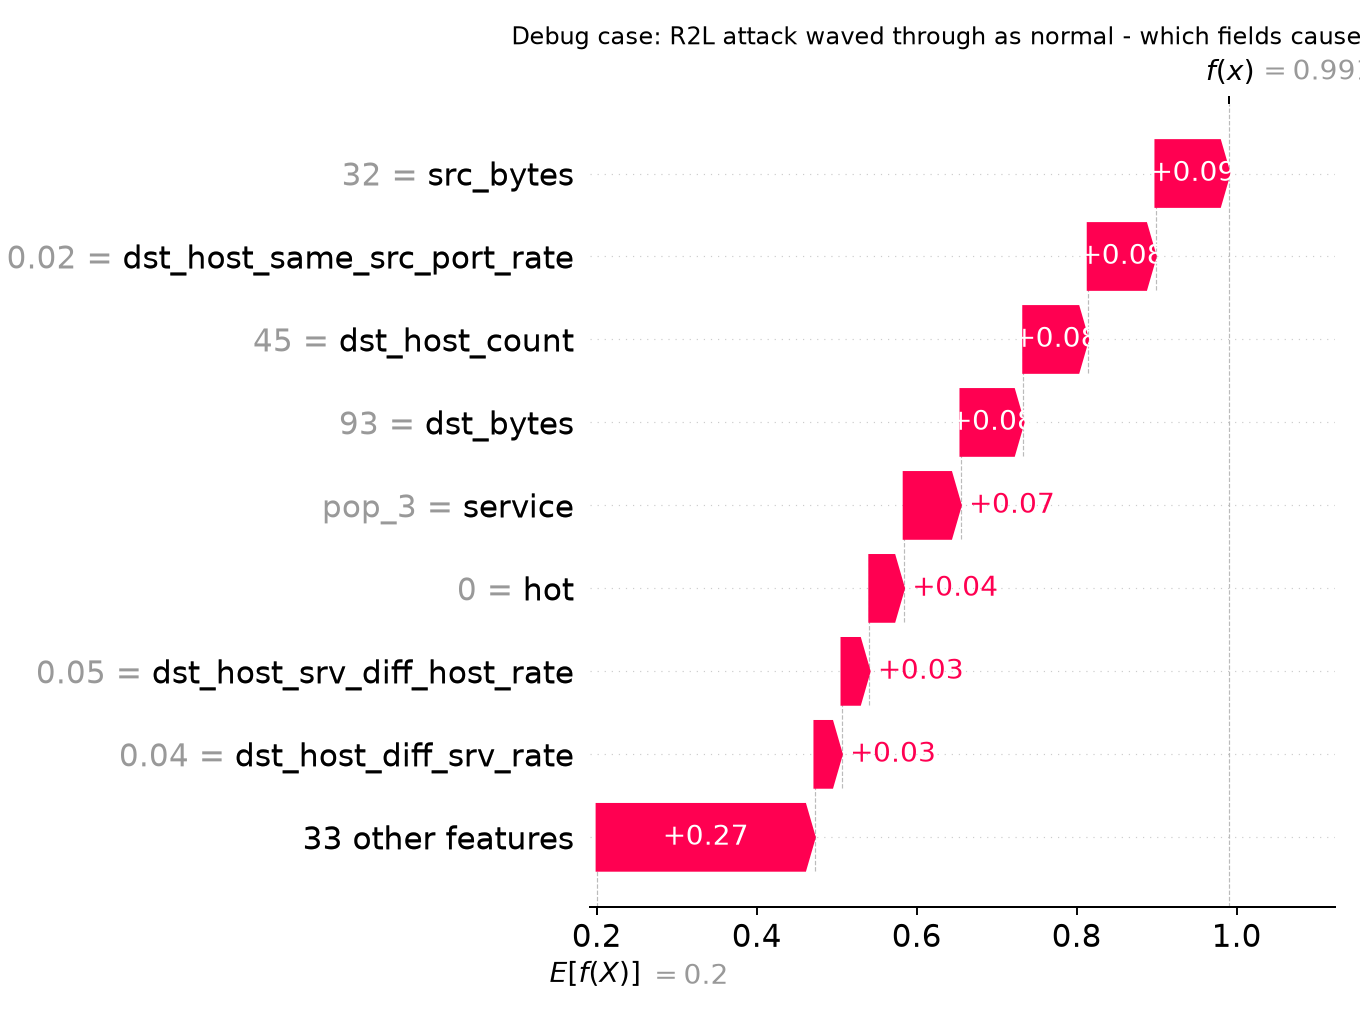
\includegraphics[width=0.98\textwidth]{../figures/local_guess_passwd.png}
\end{column}
\begin{column}{0.48\textwidth}
\scriptsize
A \f{guess\_passwd} attack waved through as \emph{normal} with $p=0.99$.

\vspace{0.6em}
\fbox{\parbox{0.95\linewidth}{\ttfamily\tiny
verdict=normal p=0.99 because\\
src\_bytes=32 (+0.092),\\
dst\_host\_same\_src\_port\_rate=0.02 (+0.085),\\
dst\_host\_count=45 (+0.081),\\
dst\_bytes=93 (+0.078)}}

\vspace{0.6em}
The verdict rests entirely on \emph{size and host counters} -- a small, ordinary
looking session. The fields that actually define this attack
(\f{num\_failed\_logins}, \f{hot}, \f{is\_guest\_login}) contribute almost
nothing, because a single credential-guessing connection looks like one
legitimate login.

\vspace{0.5em}
Actionable conclusion, obtained without new labels: per-flow features cannot
express R2L. Detection needs \textbf{cross-flow aggregation} (failed logins per
source over a time window), not a bigger model.
\end{column}
\end{columns}
\end{frame}

% ============================================================== 10. E2-E4
\begin{frame}{Result 5: which explainer should be trusted? SHAP vs LIME}
\small
\begin{columns}[T]
\begin{column}{0.47\textwidth}
\centering
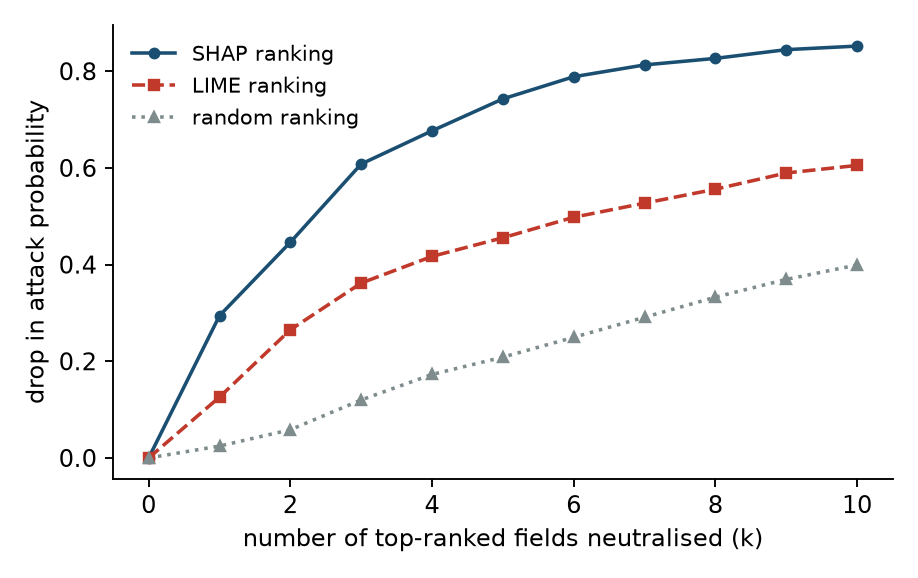
\includegraphics[width=\textwidth]{../figures/faithfulness.png}
\end{column}
\begin{column}{0.52\textwidth}
\scriptsize
\begin{tabular}{lcc}
\toprule
 & \textbf{TreeSHAP} & \textbf{LIME} \\
\midrule
Faithfulness (AOPC $\uparrow$)      & \textbf{\aopcShap} & \aopcLime \\
\quad random-ranking baseline       & \multicolumn{2}{c}{\aopcRand} \\
Stability, top-5 Jaccard $\uparrow$ & \textbf{\stabShap} & \stabLime \\
Cost per flow                       & \msTree\,ms & \msLime\,ms \\
\bottomrule
\end{tabular}
\vspace{0.5em}

KernelSHAP on the MLP (model-agnostic, 256 samples): \msKernel\,ms per flow.

\vspace{0.8em}
\begin{itemize}\itemsep3pt
  \item Neutralising only the \textbf{top-3} SHAP fields removes
        \dropTopThree{} of the attack probability; the random ranking needs all
        10 to reach less than half of that.
  \item The two methods largely \emph{disagree} on the same decision (top-5
        Jaccard \jacSL, Spearman \rhoSL). Both cannot be right -- E2 breaks the
        tie in favour of SHAP, matching Warnecke et al.\ (2020).
  \item LIME's re-sampling makes one in three top-5 fields change between
        identical runs. An incident report that changes when you press refresh
        is not evidence.
  \item Tens of ms/flow: fine for triage in a SOC console or for sampled
        traffic, far too slow inline on a 10\,Gb/s link.
\end{itemize}
\end{column}
\end{columns}
\end{frame}

% ============================================================== 11. takeaways
\begin{frame}{Takeaways and limitations}
\small
\textbf{Takeaways}
\begin{itemize}\itemsep2pt
  \item Attributions on flow data reproduce textbook attack signatures, which is
        what makes a block decision defensible to a network engineer.
  \item Explanations are also a \emph{diagnostic}: alignment lift correlated
        \corrAlign{} with recall on unseen attacks, and pointed to a concrete fix
        (cross-flow features for R2L) instead of a bigger model.
  \item Choose the explainer on evidence, not popularity: exact TreeSHAP was
        both more faithful (\aopcShap{} vs \aopcLime) and fully reproducible
        (\stabShap{} vs \stabLime).
  \item Aggregating one-hot columns back to protocol fields costs nothing
        (additivity) and is what makes the output readable.
\end{itemize}
\vspace{0.4em}
\textbf{Limitations}
\begin{itemize}\itemsep2pt
  \item NSL-KDD flow features are from 1999 traffic; CICIDS2017 with modern
        encrypted traffic is the natural next step (loader is the only change).
  \item The deletion test uses a benign-median reference, which is close to
        TreeSHAP's implicit background -- a mild bias in SHAP's favour; a
        marginal-resampling variant should be checked.
  \item Functionally-grounded metrics only; no study of whether operators
        actually make better decisions with these reasons (Doshi-Velez \& Kim).
  \item Post-hoc explanations can be attacked (Slack et al., AIES 2020) --
        an adversary aware of the explainer is out of scope here.
\end{itemize}
\end{frame}

% ============================================================== 12. links
\begin{frame}{Code, data and references}
\small
\textbf{Code (all results in this deck are reproduced by \f{run\_all.sh})}\\
\link{https://github.com/Wangzx9908/ai-hw-SUMMER-2026-MRP}{github.com/Wangzx9908/ai-hw-SUMMER-2026-MRP}
\vspace{0.3em}
\scriptsize
\begin{itemize}\itemsep0pt
  \item \f{src/dataset.py} loading, one-hot encoding, group map $\cdot$
        \f{src/train.py} RF + MLP
  \item \f{src/explain.py} TreeSHAP global/local figures, reason strings $\cdot$
        \f{src/xai\_eval.py} E1--E4 $\cdot$ \f{src/report.py} figures and slide numbers
\end{itemize}

\vspace{0.5em}
\normalsize\textbf{Data and libraries}
\scriptsize
\begin{itemize}\itemsep0pt
  \item NSL-KDD: \link{https://www.unb.ca/cic/datasets/nsl.html}{unb.ca/cic/datasets/nsl.html}
  \item CICIDS2017 (future work): \link{https://www.unb.ca/cic/datasets/ids-2017.html}{unb.ca/cic/datasets/ids-2017.html}
  \item SHAP \link{https://github.com/shap/shap}{github.com/shap/shap} $\cdot$
        LIME \link{https://github.com/marcotcr/lime}{github.com/marcotcr/lime} $\cdot$
        \link{https://scikit-learn.org/}{scikit-learn}
  \item Interpretable ML book: \link{https://christophm.github.io/interpretable-ml-book/}{christophm.github.io/interpretable-ml-book}
\end{itemize}

\vspace{0.5em}
\normalsize\textbf{Key references}
\scriptsize
\begin{itemize}\itemsep0pt
  \item Lundberg \& Lee, \emph{A Unified Approach to Interpreting Model Predictions}, NeurIPS 2017.
  \item Lundberg et al., \emph{From local explanations to global understanding with explainable AI for trees}, Nature Machine Intelligence 2020.
  \item Ribeiro et al., \emph{"Why Should I Trust You?"}, KDD 2016.
  \item Sommer \& Paxson, \emph{Outside the Closed World}, IEEE S\&P 2010.
  \item Arp et al., \emph{Dos and Don'ts of Machine Learning in Computer Security}, USENIX Security 2022.
  \item Warnecke et al., \emph{Evaluating Explanation Methods for Deep Learning in Security}, IEEE EuroS\&P 2020.
  \item Wang et al., \emph{An Explainable Machine Learning Framework for Intrusion Detection Systems}, IEEE Access 2020.
  \item Tavallaee et al., \emph{A Detailed Analysis of the KDD CUP 99 Data Set}, CISDA 2009.
  \item Nadeem et al., \emph{SoK: Explainable ML for Computer Security Applications}, IEEE EuroS\&P 2023.
\end{itemize}
\end{frame}

{\setbeamertemplate{footline}{}
\begin{frame}[plain]
\vfill
\centering
{\Large Thank you}\\[0.8em]
\small\link{https://github.com/Wangzx9908/ai-hw-SUMMER-2026-MRP}{github.com/Wangzx9908/ai-hw-SUMMER-2026-MRP}
\vfill
\end{frame}}

\end{document}
